\section{Minimalizacja w 1-D}
  \begin{frame}{Minimalizacja w 1-D}
    \begin{block}{Przydatność metod 1-D dla zag. n-D}
      \begin{itemize}
        \item prosta ilustracja ogólnych problemów
        \item metody 1-D -- często: element składowy metod n-D

      \end{itemize}

    \end{block}

  \end{frame}

\subsection{Przeglądanie siatki (grid search)}
  \begin{frame}{Przeglądanie siatki \emph{(grid search)}}
    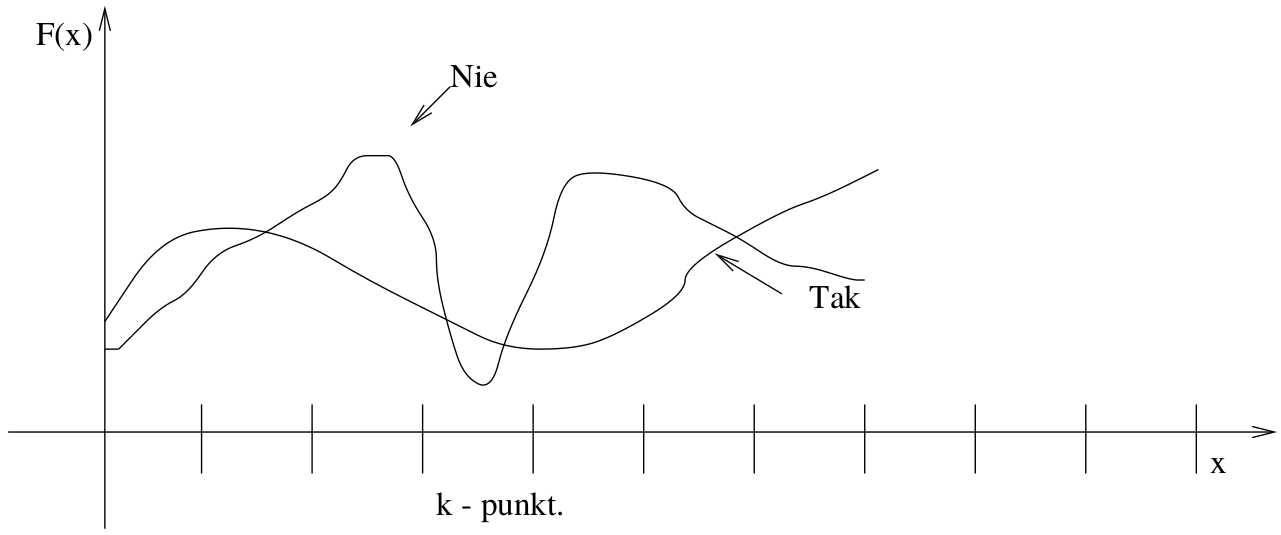
\includegraphics[width=1\textwidth]{img/17/przegladanie_siatki}
  \end{frame}

  \begin{frame}{Przeglądanie siatki \emph{(grid search)}}
    \begin{block}{Realizacja}
      \begin{itemize}
        \item przegląd wartości
        \item wybór najmniejszej $ \to $ odległości od minimum
        $ 0 \leq \frac{\Delta x}{2} $
      \end{itemize}
    \end{block}
    \begin{block}{Wady}
      \begin{itemize}
        \item nie może być stosowana dla $ \infty $ przedziału
        \item nieefektywna $ \to $ nie "uczy się", własności funkcji % there was a comma before "własności"
      \end{itemize}
    \end{block}
  \end{frame}

  \begin{frame}{Przeglądanie siatki \emph{(grid search)}}
    \begin{tabular}{@{} c l c c c @{}}
      & $ 100 $ & punktów & w & 1 -- D \\
      $ \Rightarrow $ Zawężenie obszaru do 1\% $ \Rightarrow $ & $ 100^{2} $ & & w & 2 -- D \\
      & $ 100^{10} $ & & w & 10 -- D \\
    \end{tabular}
    przy czasie obliczeń jednej wartości $F(x) \approx 10^{-5}s$
    \begin{displaymath}
      \to \text{czas obliczeń} = \frac{10^{20}*10^{-5}s}{\underbrace{\pi * 10^{7}}_{\text{sek. w roku}}} \approx 3 * 10^{7}lat \text{!}
    \end{displaymath}
    \begin{flushright}
      \emph{Zadanie:} porównaj $\to$ całki w n-D
    \end{flushright}
  \end{frame}

  \begin{frame}{Przeglądanie siatki \emph{(grid search)}}
    \begin{block}{Zalety}
      \begin{itemize}
        \item absolutna prostota
        \item bezwzględna zbieżność
        \item brak "czułości" na szczegółowe zachowanie się $F(x)$
      \end{itemize}
    \end{block}
  \end{frame}

\subsection{Metoda złotego podziału (golden section search)}
  \begin{frame}{Metoda złotego podziału \emph{(golden section search)}}
    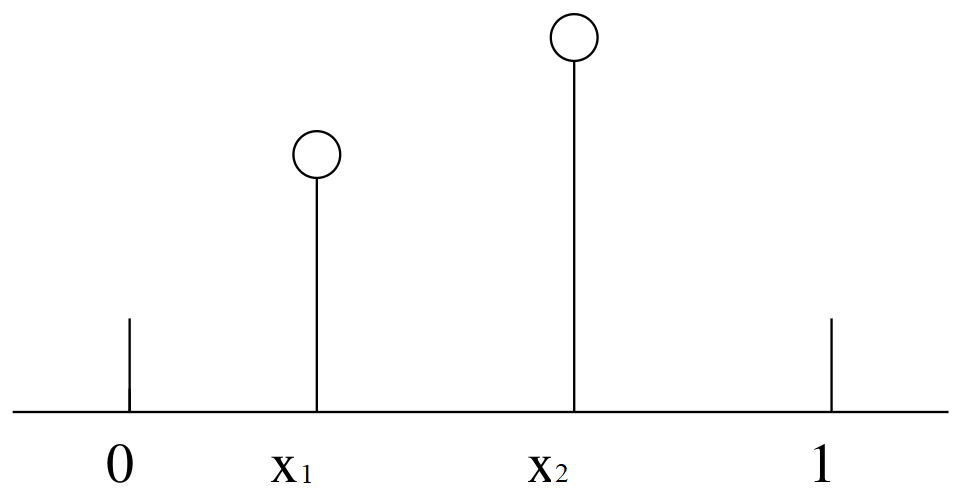
\includegraphics[width=0.9\textwidth]{img/17/f_unimodalna}
    \\
    $F(x)$ - f. unimodalna
  \end{frame}

  \begin{frame}{Metoda złotego podziału \emph{(golden section search)}}
    \begin{block}{Definicja funkcji unimodalnej}
      Funkcję $f(x)$ nazywamy \emph{unimodalną} na przedziale
      $[a{,}b]$ jeżeli:
      \begin{enumerate}
        \item $\exists x^{*}\in [a{,}b] : f(x^{*}) = min_{x \in [a{,}b]}f(x)$
        \item $\forall x_{1}{,}x_{2} : a \leq x_{1} < x_{2} \leq b$ zachodzi:
        \begin{itemize}
          \item $x_{2} \leq x_{*} \Rightarrow f(x_{1}) > f(x_{2})$
          \item $x_{1} \geq x_{*} \Rightarrow f(x_{1}) < f(x_{2})$
        \end{itemize}
      \end{enumerate}
    \end{block}
    \begin{itemize}
      \item Minimum -- w [0,1]
      \item Na początek -- potrzebne 2 punkty:
      $F(x_1),F(x_2) : F(x_1) < F(x_2) \Rightarrow \text{min} F(x)\in [0{,}x_2]$
      \item w $[0{,}x_2]$ już jest punkt $x_1$ -- dla kolejnej
      redukcji $\to$ wyznaczenie $F(x)$ tylko w jednym punkcie.
    \end{itemize}

  \end{frame}

  \begin{frame}{Metoda złotego podziału \emph{(golden section search)}}
    Rozmieszczenie punktów:\\
    $t$ -- współczynnik redukcji po każdym etapie\\
    \centering
    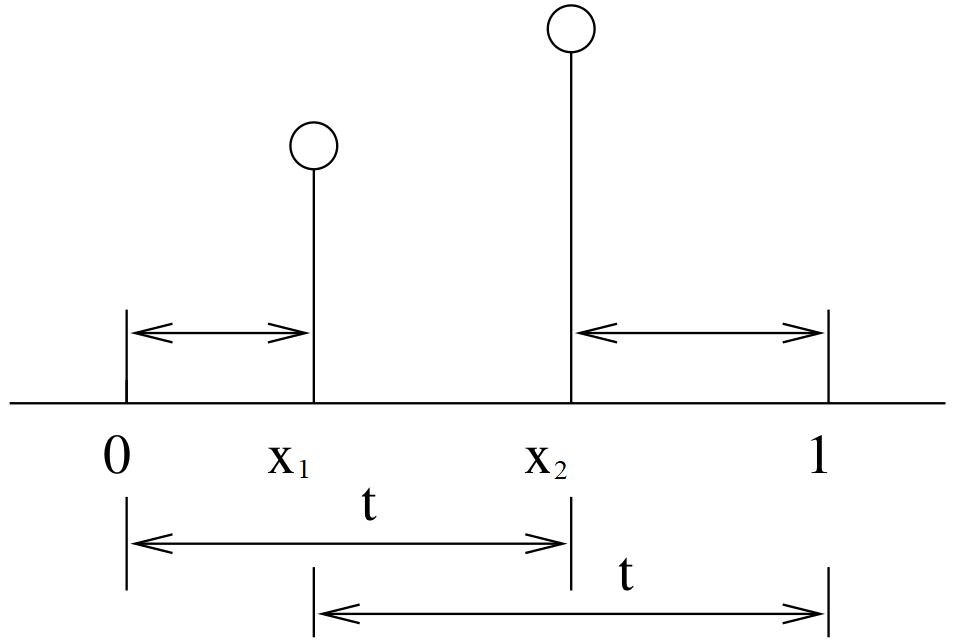
\includegraphics[height=0.6\textheight]{img/17/f_uni2}
  \end{frame}

  \begin{frame}{Metoda złotego podziału \emph{(golden section search)}}
    Po wyznaczeniu $F(x_3) \to$ długość przedziału : $t^{2}$
    \begin{displaymath}
      t^{2} = 1 - t \Rightarrow t = \frac{\sqrt{5} - 1}{2} \approx 0,616 \to \text{\emph{złoty podział}}
    \end{displaymath}
    Dla zadanej ilości kroków -- optymalna $\to$ \emph{metoda Fibonacciego}\\
    $t$ -- zmienne, (1202 króliki)\\
    \centering
    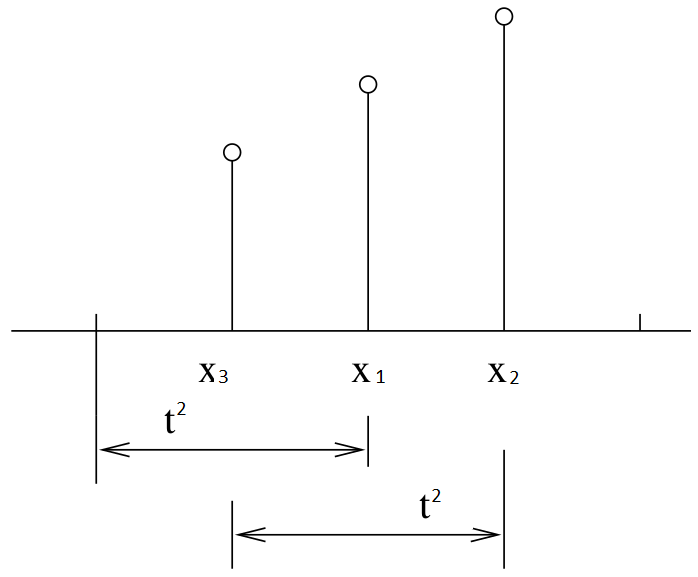
\includegraphics[height=0.55\textheight]{img/17/fibb}
  \end{frame}

  \begin{frame}{Metoda złotego podziału \emph{(golden section search)}}
    \begin{block}{Optymalność}
      W sensie minimax: minimalizuje maksymalną liczbę określeń
      $F(x)$
    \end{block}
    \begin{block}{Optymalność pesymistyczna}
      Odpowiednik najlepszej strategii w grze przeciwko
      inteligentnemu przeciwnikowi.\\
      Podejście dobre dla patologicznych funkcji.
    \end{block}
    \begin{block}{Metoda Bermana}
      $x_{0} = \frac{a + b}{2}$; poszukiwanie tam, gdzie maleje
      $\Rightarrow$ ustalony krok, w drugą stronę -- z mniejszym krokiem.
    \end{block}
  \end{frame}

\subsection{Kwadratowa interpolacja i aproksymacja}
  \begin{frame}{Kwadratowa interpolacja i aproksymacja}
    \begin{block}{Założenie: $F(x)$ jest parabolą}
      \begin{itemize}
        \item wyznaczamy $F(x)$ w 3 punktach: $x_{1}{,}x_{2}{,}x_{3}$
        (interpolacja f.~kwadr.)
        \item min $F(x) \to$ min paraboli przechodzącej przez
        $x_{1}{,}x_{2}{,}x_{3}$ znajduje się w punkcie $x_4$:
        \begin{displaymath}
          x_4 = \frac{
            \frac{F_{1}*(x_{2}+x_{3})}{(x_{1}-x_{2})*(x_{1}-x_{3})} +
            \frac{F_{2}*(x_{1}+x_{3})}{(x_{2}-x_{1})*(x_{2}-x_{3})} +
            \frac{F_{3}*(x_{1}+x_{2})}{(x_{3}-x_{1})*(x_{3}-x_{2})}
          }{2 * \left[
            \frac{F_{1}}{(x_{1}-x_{2})*(x_{1}-x_{3})} +
            \frac{F_{2}}{(x_{2}-x_{1})*(x_{2}-x_{3})} +
            \frac{F_{3}}{(x_{3}-x_{1})*(x_{3}-x_{2})}
          \right]}
        \end{displaymath}
        \begin{flushright}
          \emph{Zadanie:} Sprawdzić ten wzór
        \end{flushright}
      \end{itemize}
    \end{block}
  \end{frame}

  \begin{frame}{Kwadratowa interpolacja i aproksymacja}
    \begin{block}{A następnie:}
      \begin{itemize}
        \item $x_{4}$ -- zastępuje jeden z $x_{1}{,}x_{2}{,}x_{3}$,
        wyznaczamy nowy $x_{4} \dots$
        \item warunek zakończenia: wartość $F(x_{4})$ bliska
        $F(x_{3})$ z zadaną dokładnością
      \end{itemize}
    \end{block}
    \begin{block}{Metoda dobra dla f. zbieżnych od kwadratowych, lecz:}
      \begin{enumerate}
        \item na każdym kroku $x_{1}{,}x_{2}{,}x_{3}$ mogą
        wyznaczać $max$ a nie $min \Rightarrow$ rozbieżność
        \item gdy $x_{1}{,}x_{2}{,}x_{3}$ -- prawie na prostej
        $\to$ duży krok:
        \begin{itemize}
          \item trudności numeryczne
          \item rozbieżność
        \end{itemize}
        \item który z poprzednich punktów odrzucić?
        \item możliwe oscylacje wokół minimum zamiast zbieżności
      \end{enumerate}
    \end{block}
  \end{frame}

    \begin{frame}{Kwadratowa interpolacja i aproksymacja}
      \begin{block}{Możliwe zabezpieczenia:}
        Zaniechanie metody przy wystąpieniu trudności.
      \end{block}
      \begin{block}{Używana:}
        W ostatniej fazie minimizacji (f.~fizyczne $\to$
        paraboliczne w pobliżu minimum).
      \end{block}
    \end{frame}

\subsection{Metoda prób i błędów (success-failure method)}
  \begin{frame}{Metoda prób i błędów \emph{(success-failure method)}}
    \begin{block}{Kompromis między}
      \begin{itemize}
        \item przeszukiwaniem na siatce
        \item kwadratowa interpolacja
      \end{itemize}
    \end{block}
    $x_{0}$ -- start point, $d$ -- initial step size
    \begin{itemize}
      \item gdy $F(x_{0} + d) < F(x_{0}) \to$ sukces:\\
      $x_{0} \to x_{0} + d,$ \\
      $d \to \alpha * d, \alpha$ -- expansion factor % was: expantion
      ($\alpha > 1, \alpha \approx 3.0$)
      \item gdy $F(x_{0} + d) > F(x_{0}) \to$ niepowodzenie: \\
      $d \to -\beta * d, \beta$ -- contraction factor
      $(\beta < 1, \beta \approx 0.4)$
    \end{itemize}
    Test jest powtarzany aż do uzyskania zmian $F(x) < \epsilon$.
  \end{frame}

  \begin{frame}{Metoda prób i błędów \emph{(success-failure method)}}
    Minimum jest zlokalizowane (bracketed), gdy po sukcesie
    -- niepowodzenie wtedy, mamy trzy punkty typu:\\ % doubts about fullstop
    \begin{center}
      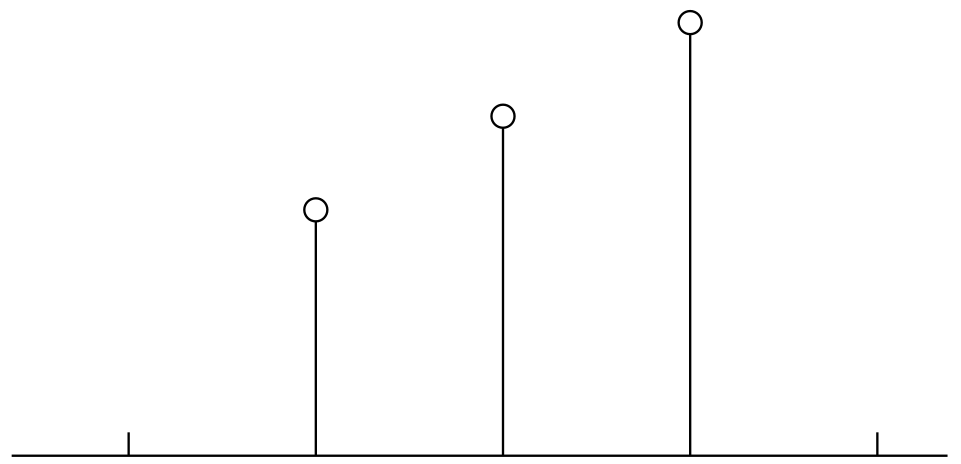
\includegraphics[width=0.7\textwidth]{img/17/s-f}
    \end{center}
    są one \emph{punktem startowym} interpolacji kwadratowej.\\
    \textbf{Uniwersalna, efektywna metoda 1-D dla ogólnych funkcji.}
  \end{frame}
